\chapter{Detail Design}\label{Ch4}
In this chapter, the detailed design of the Body Temperature Measuring Wristband will be presented. The detailed design is started with trade-off studies, where Multi-Criteria Decision Matrices (MCDM), together with user-defined utility functions are used to select the specific components required to physically construct the device. The best technique available from the literature study to estimate core body temperature from the temperature of the skin will also be determined. After the selection of components and the measurement technique, the complete circuit of the Body Temperature Measuring Wristband will be given. The design of the embedded firmware will also be presented in this chapter in the form of state machines, as well as firmware flow diagrams.

\section{Trade-off Studies}
In this section, trade-off studies will be performed to select specific components to construct the device. The components that will be selected by the trade-off studies include the temperature probe, the microcontroller, the battery, and the display. Each component will have its own set of criteria, as well as utility functions. In order to determine which component inside the MCDM is best suited, the Weighted Product Method (WPM) algorithm is used. In this algorithm, the utility value of a criterion is raised to the power of the weight of that criterion, and all these weighted scores are then multiplied together. This is done for each alternative component. The formula for WPM is given in \autoref{WPM} \cite{MCDM2020}.
\begin{equation}
    P(A_{K}) = \prod_{j = 1}^{n} (a_{Kj})^{wj}, \;for \;K = 1, 2, 3,....,m.
    \label{WPM}
\end{equation}
\noindent
In this section, the measurement technique will also be selected. This will be done through an analysis and discussion on the advantages and disadvantages of each estimation technique.

\subsection{Microcontroller}
The microcontroller serves as the central processing unit of the body temperature measuring wristband. The microcontroller will be used for communication between the different components, for all the required processing in the process of measuring body temperature, and to distribute power to the components. There are a wide variety of microcontrollers available on the market today, each having its own set of available peripherals, processing speeds, unique features, etc. Therefore, familiar microcontrollers that were available at the time the trade-off studies were conducted, are considered. For the microcontroller of the device, four possibilities were considered:
\begin{itemize}
	\item PIC24FJ64GA004:\\
	The PIC24FJ64GA004 family of microcontrollers are developed by Microchip and is 28/44-pin general-purpose, 16-bit flash microcontrollers. 
	\item PIC24FJ256GA705:\\
	The PIC24FJ256GA705 family of microcontrollers is also developed by Microchip. These are 16-bit general-purpose microcontrollers that have low-power features. 
	\item STM8L15:\\
	The STM8L15 series are developed by STMicroelectronics and are 8-bit ultra-low-power microcontrollers. 
	\item STM32L071KBT6:\\
	The STM32L07 series are also developed by STMicroelectronics and are 32-bit ultra-low-power microcontrollers.
\end{itemize}
\noindent
The evaluation criteria for selecting the microcontroller is:
\begin{itemize}[noitemsep]
	\item Technical Risk
	\item Cost per Unit
	\item Power Consumption
	\item Clock Speed
	\item Lead Time
\end{itemize} 
\noindent
The ability of the designer to correctly implement and interface the specific component with the rest of the circuitry is included in the evaluation criteria as technical risk. Power consumption will play a crucial role in the battery life of the device, and should therefore be kept as low as possible. Since the current drawn by the microcontroller will depend on the connected components, it is difficult to compare power consumption between different microcontrollers. Therefore, the power consumption of the possible microcontrollers is based on the operating current at the lowest clock speed of that microcontroller. This is done so that the microcontrollers can be compared to one another in terms of power consumption, and clock speed. The cost and lead time of the component should be kept as low as possible. Technical Risk is divided into 5 levels and is defined as shown in \autoref{fig:19}. Technical Risk will also be included in the evaluation criteria for the rest of the components and will stay as defined throughout. The utility functions for each criterion are shown in \autoref{fig:21}.
\begin{figure}[H]
	\centering
	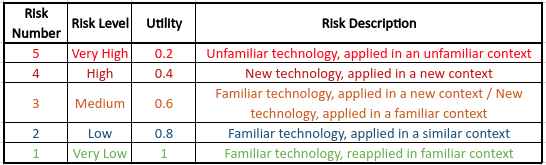
\includegraphics[scale=0.7]{img/Technical Risk}
	\caption{Technical Risk Definition}
	\label{fig:19}
\end{figure}
\begin{figure}[H]
	\centering
	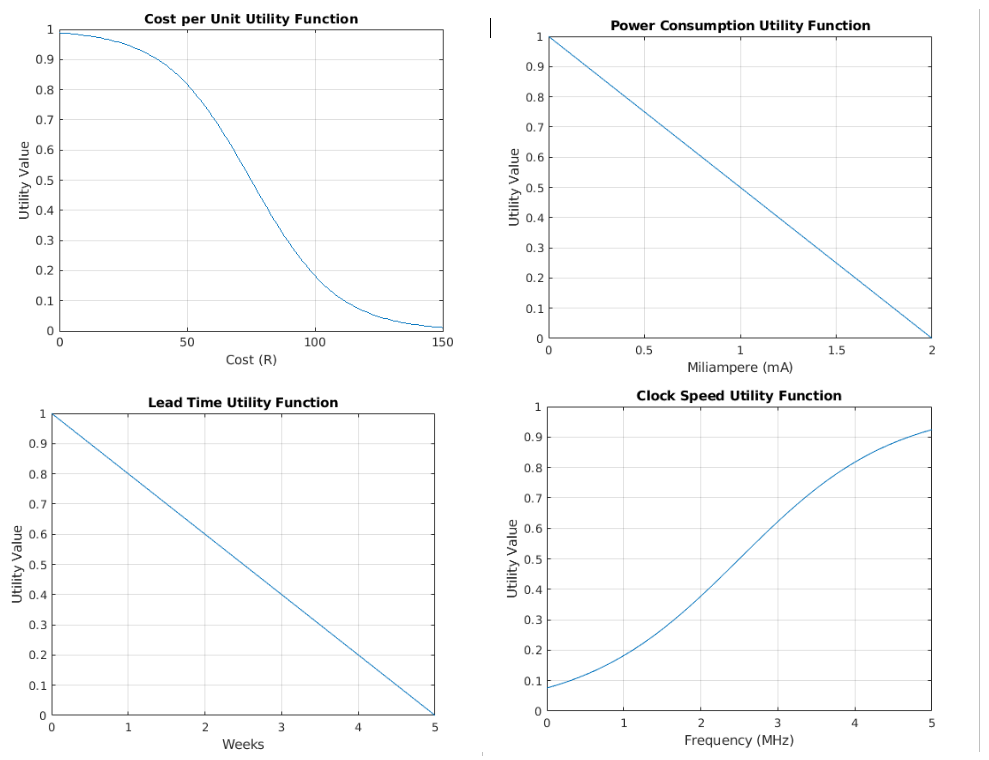
\includegraphics[scale=0.4]{img/M-Util}
	\caption{Microcontroller - Utility Functions}
	\label{fig:21}
\end{figure}
\noindent
The Multi-Criteria Decision Matrices (MCDM) for each microcontroller is shown in \autoref{fig:22}. The weights of the evaluation criteria are chosen according to the importance of the criterion. Power consumption was favoured above clock speed since clock speeds are not as important as power consumption in this energy-efficient application which does require not as much processing. The rest of the evaluation criteria have the same weight as they are of equal importance. All the technical values are obtained from the respective data sheets, the cost is included without tax or shipping to compare the basic microcontroller cost, and the lead time includes shipping. 
\begin{figure}[H]
	\centering
	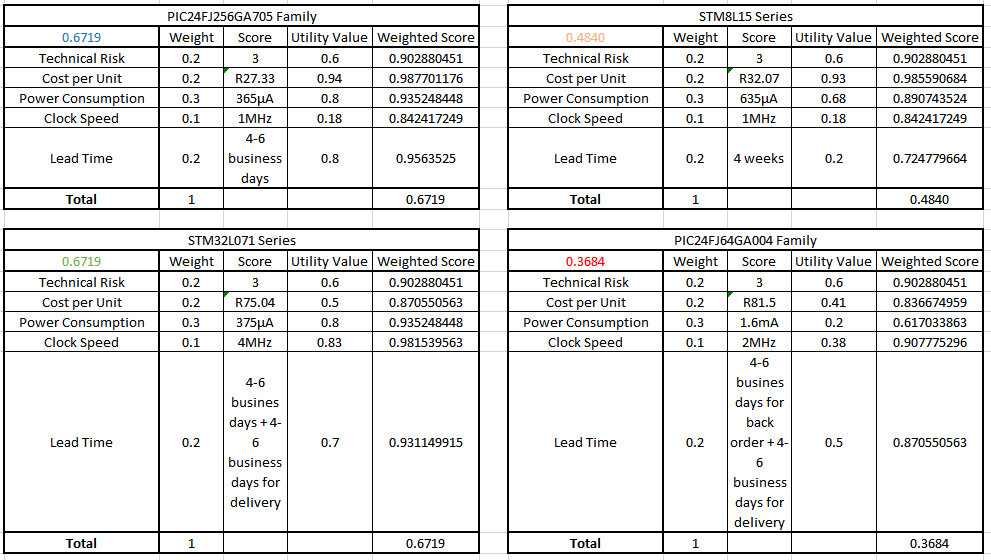
\includegraphics[scale=0.55]{img/M-MCDM}
	\caption{Microcontroller - MCDM}
	\label{fig:22}
\end{figure}
\noindent
From the trade-off study, it is clear that the STM32L071, as well as the PIC24FJ256GA705 series of microcontrollers, are equally suited for this application. The decision is therefore made to use the STM32L071. More specifically, the STM32L071KBT6 of this series will be used. The decision is simply based on preference between STM and PIC microcontrollers.  This microcontroller includes two I2C peripherals, Analog to Digital converters (ADC), Real-Time Clock (RTC) functionality, 128K bytes for program memory, and 20K bytes for RAM. This device has 32 pins, where 25 of them are available for GPIO (General Purpose Input/Output), which will be used for display and input purposes. The STM32L071KBT6 features low power consumption in run mode, and has ultra-low power modes available such as Standby mode (0.29$ \mu $A), Stop mode (0.43$ \mu $A), and Stop mode with RTC (0.86$ \mu $A).

\subsection{Temperature Probe}
The temperature probe will be used to measure the body temperature of the user. For the temperature probe, four possibilities were considered. All of these possibilities have a measurement range that includes the required range for body temperature, and since the chosen microcontroller has many peripherals available, the options may use any possible interface to communicate. The possible temperature probes are:
\begin{itemize}
	\item LM35:\\
	The LM35 is an analog temperature sensor that has an output voltage directly proportional to the measured temperature. 
	\item TMP117:\\
	The TMP117 is a digital temperature sensor integrated circuit (IC) that uses the I2C/SMBus communication protocol.
	\item DS18B20:\\
	The DS18B20 is a digital thermometer that utilises 1-Wire technology for communication with a microprocessor. 
	\item MAX30205:\\
	The MAX30205 is an accurate, low-voltage digital temperature sensor that uses the I2C protocol for communication.
\end{itemize}
\noindent
The evaluation criteria for selecting the temperature probe is:
\begin{itemize}[noitemsep]
	\item Technical Risk.
	\item Measurement Accuracy.
	\item Cost per Unit.
	\item Power Consumption.
	\item Lead Time.
\end{itemize}
\noindent
Since body temperature plays a crucial role in one's health, it must be measured accurately. Therefore, the measurement accuracy of the temperature sensor is included in the criteria. The sensor cost and lead time must be kept as low as possible, as well as the power consumption since the device will be battery operated. The utility functions for each criterion are now given and are shown in \autoref{fig:18}.
\begin{figure}[H]
	\centering
	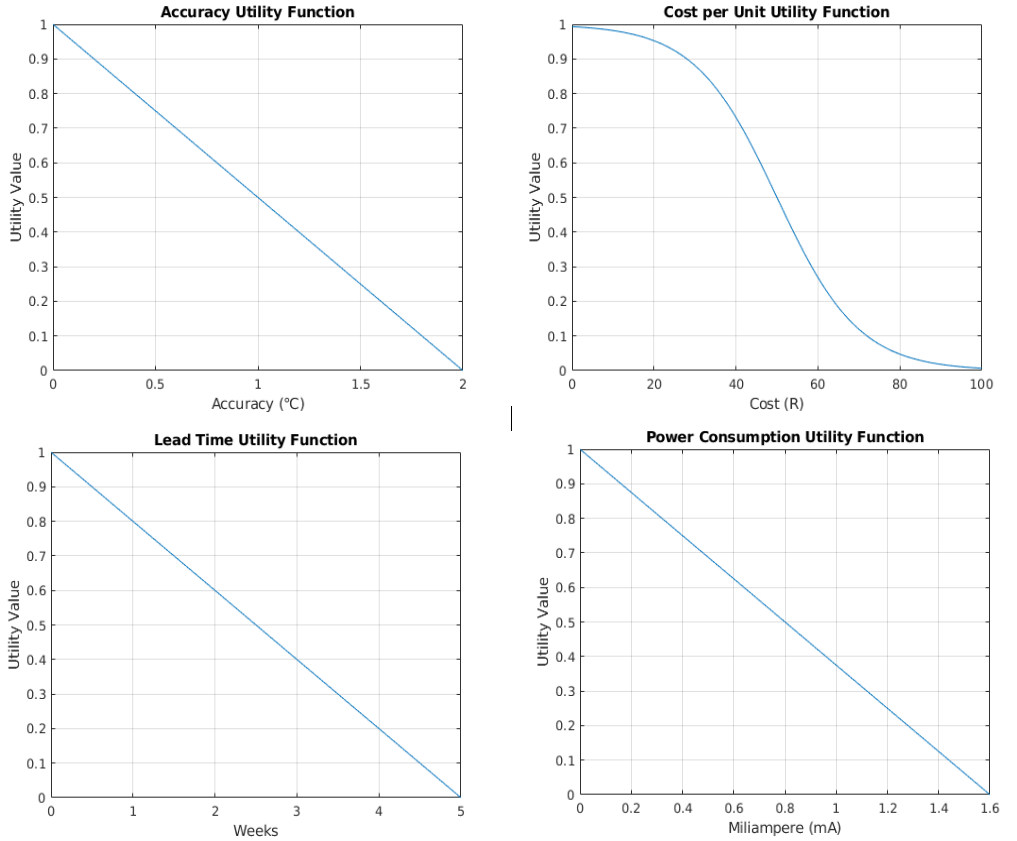
\includegraphics[scale=0.4]{img/T-Util}
	\caption{Temperature Probe - Utility Functions}
	\label{fig:18}
\end{figure}
\noindent
The Multi-Criteria Decision Matrices (MCDM) for each possibility is shown in \autoref{fig:20}. The weights of the evaluation criteria are chosen the same since all the criteria are of equal importance when choosing the temperature probe. All the technical values are obtained from the respective data sheets, the cost is included without tax or shipping to compare the basic sensor cost, and the lead time includes shipping.
\begin{figure}[H]
	\centering
	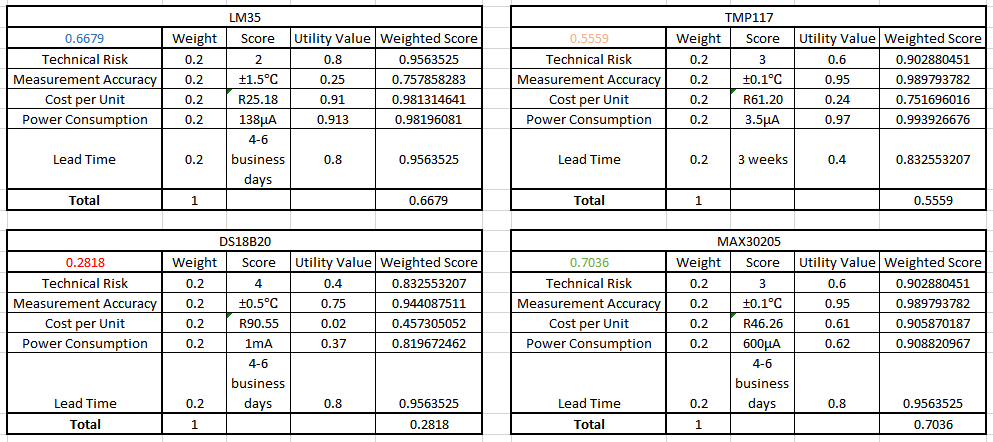
\includegraphics[scale=0.55]{img/T-MCDM}
	\caption{Temperature Probe - MCDM}
	\label{fig:20}
\end{figure}
\noindent
Therefore, the temperature probe that will be used is the MAX30205 digital temperature sensor. 

\subsection{Display}\label{disp}
The display will show the user the measured body temperature, as well as the current time of day. The display will also be used by the user to configure the device. There are various types of displays on the market, ranging from touch screens to LED matrix displays, all coming in a wide variety of sizes. The displays that are considered must be compact and small, energy-efficient, and touch screen are not required. In the case where a driver IC is needed by the display, only the displays that come with the required IC built-in were considered since they do not require any external components or configurations to work properly. For the display of the device, four possibilities were considered:
\begin{itemize}
	\item 0.91 Inch OLED Display Module:\\
	This is an OLED display with 128x32 pixels that comes with an embedded controller that communicates via the I2C interface. 
	\item 4 Digit 7-Segment LED Display:\\
	This is a display consisting of four standard 7-segment displays that are connected together in one package.  
	\item Midas 0.49in White Passive Matrix OLED Display:\\
	This is a 64x32 resolution OLED display that has a white-on-black appearance, that also comes with an embedded controller that communicates via I2C.
	\item RS PRO TFT LCD Colour Display:\\
	This display is a full-colour TFT LCD module with a normally white backlight. The screen has a 160x80 resolution and the display communicates via a 3- or 4-wire serial peripheral interface.
\end{itemize}
\noindent
The evaluation criteria for selecting the display is:
\begin{itemize}[noitemsep]
	\item Technical Risk.
	\item Size of the Module.
	\item Cost per Unit.
	\item Power Consumption.
	\item Lead Time.
\end{itemize}
\noindent
The size of the display will play a crucial role in the overall size of the final device and should be kept as small, yet as legible as possible since the device will be in the form of a wristband. The device will be battery operated, and the power consumption by the display should be as low as possible in order to provide longer battery life. The cost and lead time should, once again, be as low as possible. The utility functions for each criterion are shown in \autoref{fig:25}.
\begin{figure}[H]
	\centering
	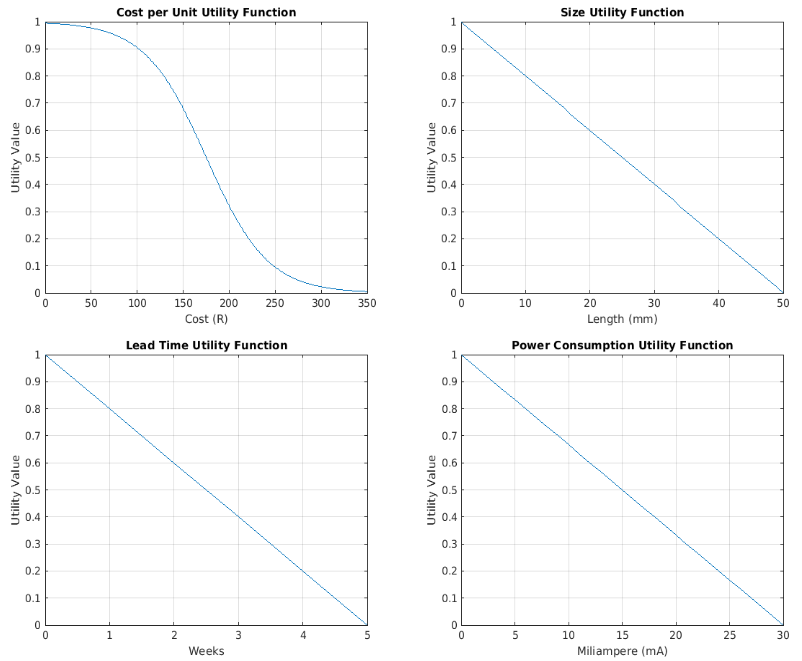
\includegraphics[scale=0.5]{img/D-Util}
	\caption{Display - Utility Functions}
	\label{fig:25}
\end{figure}
\noindent
The Multi-Criteria Decision Matrices (MCDM) for each possibility is shown in \autoref{fig:26}. All the technical values are obtained from the respective data sheets, the cost is included without tax or shipping to compare the basic sensor cost, and the lead time includes shipping. The weights of the evaluation criteria are chosen the same since all the criteria are equally important. Although the size of the screen plays a very important role, it cannot have a higher weight than the other criteria since they are of equal importance.
\begin{figure}[H]
	\centering
	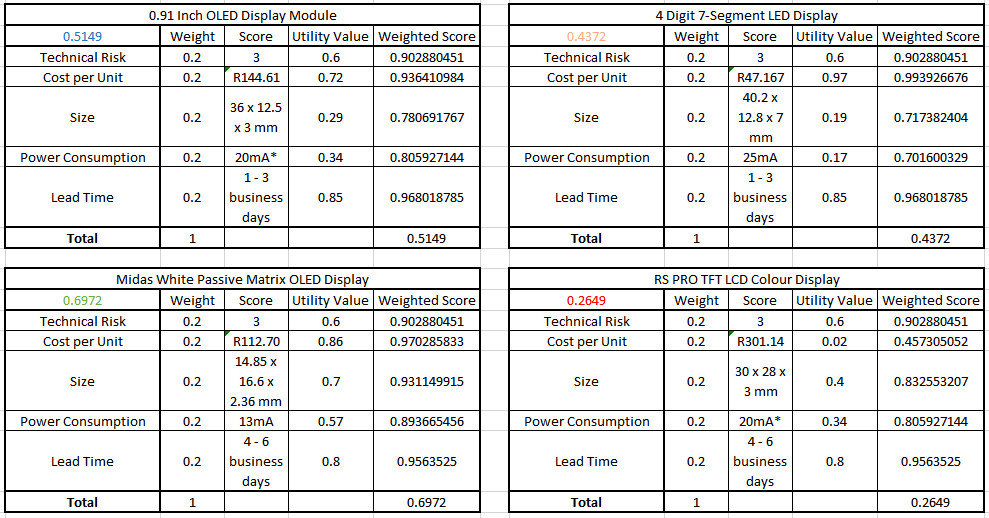
\includegraphics[scale=0.55]{img/D-MCDM}
	\caption{Display - MCDM}
	\label{fig:26}
\end{figure}
\noindent
From the trade-off study, it is clear that the White Passive Matrix OLED Display from Midas will be best suited for the body temperature measuring device. As mentioned previously, this display has a 64x32 resolution and has the SSD1306 controller built-in on the display module, and communicates via the I2C interface. 


\subsection{Battery} 
The battery will provide power to the microcontroller, as well as the other components of the device. For the battery, two different possibilities that are easily accessible were considered:
\begin{itemize}
	\item RS PRO LIR2032:\\
	This is a rechargeable button battery with a chemical composition of Lithium-ion.
	\item RS PRO Lithium Polymer battery:\\
	This is a Li-Polymer rechargeable battery that has a low self-discharge and comes pre-wired with bare wire terminals.
	\item Panasonic CR2032 Button battery:\\
	This is a non-rechargeable coin cell battery that have a low self-discharge rate.
\end{itemize}
\noindent
The evaluation criteria for selecting the battery is:
\begin{itemize}[noitemsep]
	\item Technical Risk
	\item Cost per Unit
	\item Size
	\item Capacity
	\item Lead Time
\end{itemize}
\noindent
Since the developed device will be in the form of a wristband, the size of the product must be small, to provide maximum comfort. In order to compare the button batteries to the battery that has a square shape, only the length of each will be considered. The capacity of the battery will determine how long the body temperature wristband will last, and therefore, the higher the capacity, the better. As previously, the cost and lead time should be as low as possible. The utility functions for each criterion for the battery are shown in \autoref{fig:23}, and the Technical Risks are defined once again as in \autoref{fig:19}.
\begin{figure}[H]
	\centering
	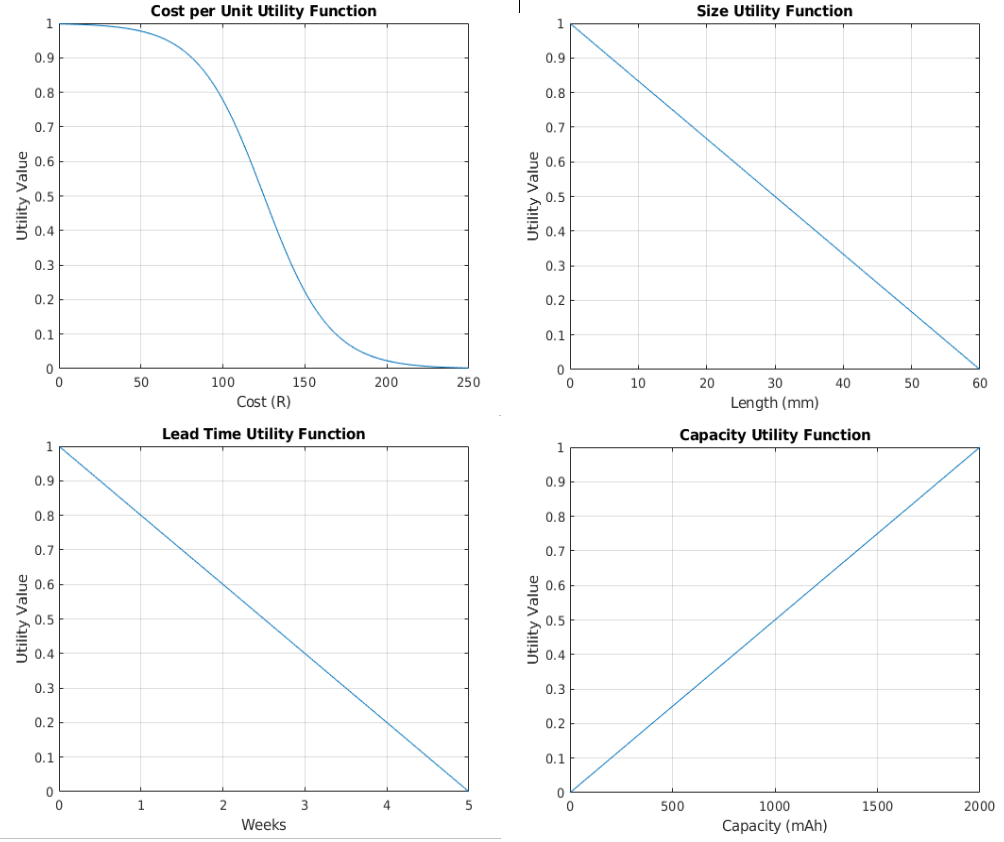
\includegraphics[scale=0.4]{img/B-Util}
	\caption{Battery - Utility Functions}
	\label{fig:23}
\end{figure}
\noindent
The Multi-Criteria Decision Matrices (MCDM) for each battery is shown in \autoref{fig:24}. Capacity and size are favoured in terms of the evaluation weight above the other criteria since they are of most importance in choosing the battery. Technical Risk is given a lower weight as the use of batteries is straightforward, although battery management and recharging may be more complex. Lead time is also given a lower weight since batteries are relatively easily accessible. The cost is included without tax or shipping to compare the basic battery cost, the lead time includes shipping, and all the technical values are obtained from the respective datasheets.
\begin{figure}[H]
	\centering
	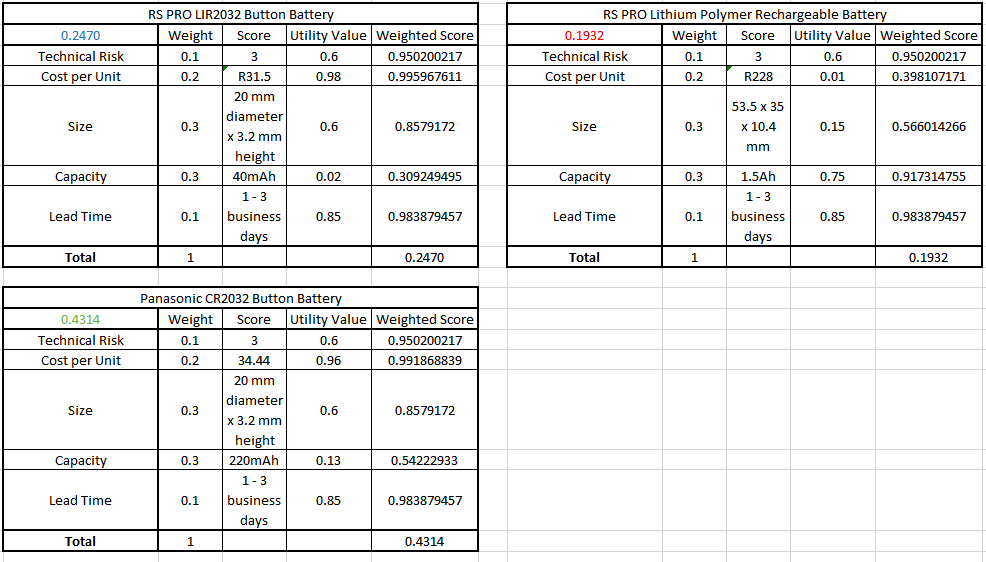
\includegraphics[scale=0.55]{img/B-MCDM}
	\caption{Battery - MCDM}
	\label{fig:24}
\end{figure}
\noindent
Therefore, the battery that will be used is the Panasonic CR2032 Button battery. This battery is non-rechargeable as mentioned previously, and it has a nominal voltage of 3.0V. The nominal voltage of the battery will be sufficient to power the microcontroller, which has a supply voltage range of 1.65V to 3.6V. This nominal voltage is also sufficient to power the temperature probe which has a 2.7V to 3.3V supply voltage rating, and the display, which can be powered from 2V to 5V. The big advantage of this battery is that no extra recharging circuitry, which will consume a lot of space, is needed. This type of battery is also commonly available in grocery stores, garages, etc. making it easily accessible when it must be replaced. 

\subsection{Measurement Technique}\label{technique}
In \autoref{Sec2_4} of this report, several non-invasive techniques to measure core body temperature from skin temperature were introduced. To determine which of these methods will be best suited to implement on the Body Temperature Monitor, a less analytical method than previous, are followed. The advantages, as well as disadvantages of each technique, are compared to one another, to determine which technique is best suited. The advantages and disadvantages of each technique are summarised below.
\begin{itemize}
    \item Zero-heat-flow:\\
    Advantage(s): Estimates Core Body Temperature accurately.\\
    Disadvantage(s):  Heater element consumes a lot of power. Extra components are needed (Heater, Thermal insulator, 2x Thermistors).
    
    \item Dual-heat-flux:\\
    Advantage(s): Estimates Core Body Temperature accurately, while using less energy than the zero-heat-flow method.\\
    Disadvantage(s): Four temperature probes are needed. Long measurement time. Systems based on this method are relatively large.
    
    \item Thermal Equivalent Circuit:\\
    Advantage(s): Estimates Core Body Temperature accurately, and takes ambient temperature into consideration. \\
    Disadvantage(s): Requires the thermal resistance of the body, which may differ from person to person. This method also requires that the probe is wrapped in a highly thermally conductive material.
    
    \item Statistical Estimation:\\
    Advantage(s): Estimates Core Body Temperature accurately, whilst taking ambient conditions and different skin types into consideration in the development of the statistical model. \\
    Disadvantage(s): This technique will require a lot of data or samples to build an accurate and reliable statistical modal.
\end{itemize}
\noindent
All of the techniques mentioned above estimates Core Body Temperature relatively accurately, and ambient conditions are accounted for within each technique. Therefore, to determine which technique is best, the disadvantages of each technique will be compared to each other. 
\\
\\
The device must be energy efficient, hence it can be concluded that the zero-heat-flow method is not the best-suited technique for this application, since the heater element used in this technique will consume a lot of power. The dual-heat-flux may result in a device that is relatively large in size, and also more expensive since four temperature probes are required. The thermal equivalent circuit model requires the thermal resistance of the body. The thermal resistance may differ from person to person, and from skin to skin, which may result in inaccurate temperature readings for some people. Therefore, the best technique for this application is a statistical estimation. Although this technique requires a lot of data to build an accurate statistical model, no extra components are needed, the size of the device can be kept as small as possible, and it will be the most energy-efficient measurement technique to use for this application. Since the technique is based on statistical models, which can be improved by gathering more data, the accuracy of the device can be improved even after it is physically constructed.

\section{Physical Architecture}
In this section the updated physical architecture of the Medical Wristband Body Temperature Monitor is shown. The components from the trade-off studies in the previous section are added to the diagram, as well as some interfaces between the components. The detailed physical architecture of the device is shown in \autoref{fig:27}.
\begin{figure}[H]
	\centering
	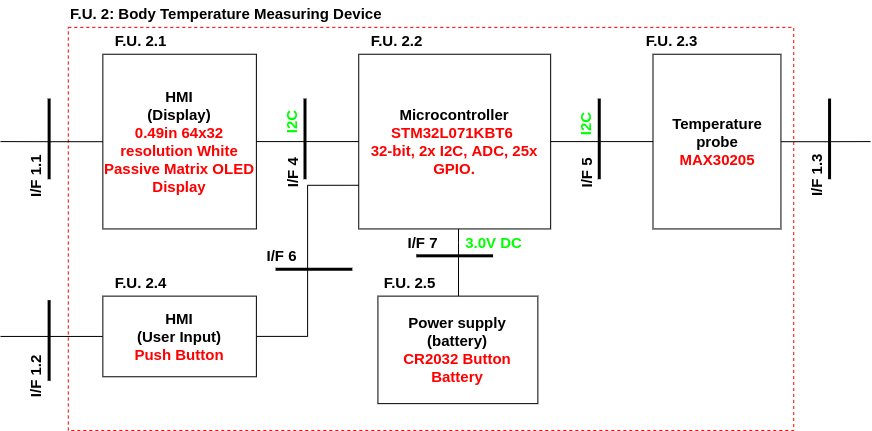
\includegraphics[scale=0.5]{img/Detail_PA}
	\caption{Detailed Physical Architecture}
	\label{fig:27}
\end{figure}


\section{Schematics}
This section will show the schematics for the Body Temperature Measuring device. The schematic of the device will be broken down into sub-systems to aid legibility, however, the full schematic can be found in \autoref{FSchematic}. The sub-systems for the Body Temperature Measuring device are as follow:
\begin{itemize}[noitemsep]
	\item The Microcontroller and all relevant components.
	\item The Temperature sensor and all relevant components.
	\item The user input buttons.
	\item The Power supply unit.
	\item External component connectors.
\end{itemize}

\subsection{Microcontroller}
This section will show the schematic for the microcontroller of the device. All the components related to the microcontroller, such as decoupling capacitors, resistors, etc. are also shown in the schematic. The microcontroller and relevant circuits can be referred to as the processing unit of the device. The schematic for the processing unit of the device is shown in \autoref{fig:28}. 
\begin{figure}[H]
	\centering
	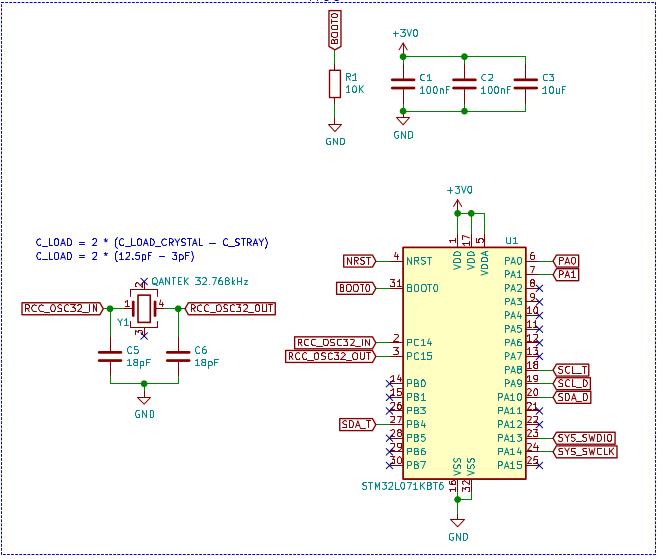
\includegraphics[scale=0.6]{img/Schematic_MCU}
	\caption{Schematic: Microcontroller}
	\label{fig:28}
\end{figure}
\noindent
From \autoref{fig:28} all the connections to and from the microcontroller can be seen as the connections are labelled. These labels show the physical connections to all the other components of the device, as two labels with the same value are connected.  
\\
\\
\autoref{fig:28} shows that there are three decoupling capacitors for the microcontroller. From the datasheet of the STM32L071KBT6, ST recommends that for every $ V_{DD} $ and $ V_{SS} $ pair of the microcontroller, a $ 100 nF $ capacitor is needed. They also recommend that in addition to the $ N \times 100 nF $ capacitors, one $ 10 \mu F $ capacitor is needed. It can be seen that the $ BOOT0 $ pin of the microcontroller is pulled to ground via a resistor. This is done to hold the logic level near 0V on this pin. The $ BOOT0 $ pin must be at the defined low logic level (ground) to select the main flash memory as the boot space of the microcontroller. 
\\
\\
A low-speed external (LSE) crystal oscillator is also connected to the microcontroller. This crystal oscillator will be used as the frequency source of the RTC. The microcontroller features a low-speed internal RC oscillator that may be used for this purpose, but internal low-speed clocks tend to have a low accuracy, which is not ideal for time-keeping purposes. The decision is therefore made to add a $ 32.768 kHz $ external crystal oscillator to the microcontroller. This value of $ 32.768 kHz $ is commonly used as the frequency in RTC applications since it is a power of 2 ($ 2^{15} $) value and one can get a precise 1 second period ($ 1 Hz $) by using a 15 stage binary counter. Sometimes, a feed resistor is needed between the oscillator and the microcontroller. A feed resistor limits the amount of drive going to and from the crystal ensuring that the crystal waveform is not distorted. However, ST strongly recommends not to add an external resistor between the oscillator pins of the microcontroller. Two load capacitors can be seen at the crystal oscillator. The values of the load capacitors are calculated by using the following formula:
\begin{equation}
C_{load} = 2 \times (C_{crystal} - C_{stray})
\end{equation}
\noindent
Where $ C_{crystal} $ is the load capacitance of the crystal which is found in the datasheet as $ 12.5 pF $, and $ C_{stray} $ is the stray capacitance of the PCB which is assumed as $ 3 pF $. Therefore, $ 19 pF $ is the calculated value of the load capacitors, and the nearest commercial capacitor value that could be found is $ 18 pF $.

\subsection{Temperature Sensor}
This section will show the schematic for the temperature sensor of the device. The schematic for the MAX30205 temperature sensor is shown in \autoref{fig:29}.
\begin{figure}[H]
	\centering
	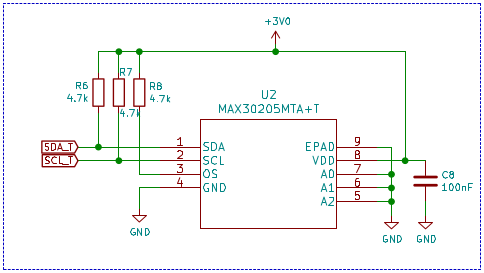
\includegraphics[scale=0.6]{img/Schematic_Temp}
	\caption{Schematic: Temperature sensor}
	\label{fig:29}
\end{figure}
\noindent
From \autoref{fig:29} it can be seen that three pull-up resistors are needed, one for the Serial Clock Line (SCL), one for Serial Data Line (SDA), and one for Over-temperature Shut-down (OS). It can also be seen that a $ 100 nF $ capacitor is needed between $ V_{DD} $ and ground. This is obtained from an application circuit in the MAX30205 datasheet. This temperature sensor communicates via I2C and in \autoref{fig:29} it shows that the MAX30205 are connected to pins 18 (SCL) and 27 (SDA) of the microcontroller. Since $ A0 $, $ A1 $, and $ A2 $ are all connected to ground, the slave address in hex of the temperature sensor is 90h.
 
\subsection{User Input buttons}
The user input buttons will be used to wake the device from standby mode, as well as to change what is being displayed by the device. The device will also be configured by one of the input buttons. The schematics for the two input buttons are shown in \autoref{fig:30}.
\begin{figure}[H]
	\centering
	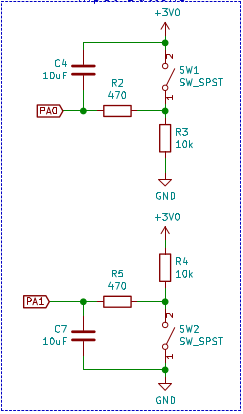
\includegraphics[scale=0.7]{img/Schematic_Button}
	\caption{Schematic: Input Buttons}
	\label{fig:30}
\end{figure}
\noindent
From \autoref{fig:30} it can be seen that one of the input buttons of the device has an active-high configuration, whilst the other input button has an active-low configuration. The active-high button is used to wake the microcontroller from standby or low-power mode. This needs to be an active-high configuration since the device will only wake on the rising edge of any of the three wake-up (WKUP) pins. Pin 6 (PA0) is used in this case to wake the device. The active-low button is used as an input button so that the user can change what is being displayed by the device, and also set the current time and date, etc. The reason an active-low configuration is used to capture the input of the user is to ensure that it is functional if and only if an intentional logic state is applied. Therefore, ambiguous floating input conditions are avoided in the process. The input button is connected to pin 7 (PA1) of the microcontroller.
\\
\\
It can also be seen that both the buttons have a de-bouncing circuit. This is to deal with the mechanical bounce of the switch contacts after they are hit together (button was pressed) since most microcontrollers will interpret this bouncing action as separate hits of the button.

\subsection{Power Supply}
This section will show the power supply of the body temperature measuring device. The device will be battery operated as mentioned previously. The power supply of the device is shown in \autoref{fig:31}.
\begin{figure}[H]
	\centering
	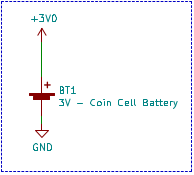
\includegraphics[scale=0.7]{img/Schematic_Battery}
	\caption{Schematic: Power Supply}
	\label{fig:31}
\end{figure}
\noindent
From \autoref{fig:31} it can be seen that the power supply of the device is just a single coin cell battery. No voltage regulator is required since all of the components of the device have an input voltage range that includes the 3V being delivered by the battery. 

\subsection{External Component Connectors}
The display, as well as the flash programmer, must connect to the device externally. This section will show the schematics for the external component connectors.
\subsubsection{Display Connector}
Although the display is part of the body temperature measuring device, it will be connected externally to the device since the display is in the form of a module. The connection between the display and the main circuit of the body temperature device will be made through header pins. Therefore, to ensure communication between the microcontroller and the display, it must be accommodated for in the schematic. The display that will be used (determined in \autoref{disp}) has the following pinout as obtained from the datasheet:
\begin{table}[H]
	\centering
	\caption{\textit{Display pinout}}
	\label{tab:4}
		\begin{tabular}{|c|c|}
		\hline
		\textbf{Pin} & \textbf{Symbol}\\
		\hline
		\hline
		1 & GND\\
		\hline
		2 & VCC\\
		\hline
		3 & SCL\\
		\hline
		4 & SDA\\
		\hline
	\end{tabular}
\end{table}
\noindent
The schematic for the display connector is shown in \autoref{fig:32}. The display communicates to the microcontroller via the I2C interface, and it will be connected to pins 19 (SCL) and 20 (SDA) of the microcontroller via the display connector..
\begin{figure}[H]
	\centering
	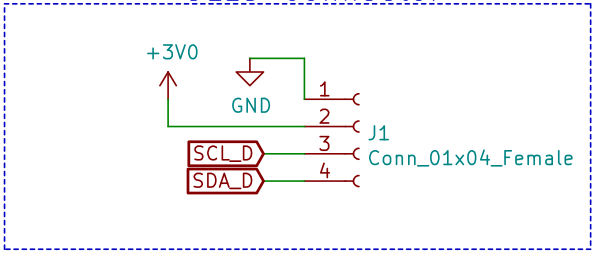
\includegraphics[scale=0.6]{img/Schematic_Disp}
	\caption{Schematic: Display Connector}
	\label{fig:32}
\end{figure}
\subsubsection{Flash Connector}
The Flash connector or from now on SWD (Serial Wire Debug) connector, will be used to flash program code onto the microcontroller. An ST-LINK/V2-1 will be used to flash the code onto the device. The ST-LINK that will be used has the following pinout, which shows the required connections to the microcontroller in order to flash program code on to the device:
\begin{table}[H]
	\centering
	\caption{\textit{SWD Connector}}
	\label{tab:5}
	\begin{tabular}{|c|c|c|}
		\hline
		\textbf{Pin} & \textbf{Symbol} & \textbf{Designation}\\
		\hline
		\hline
		1 & VDD\_Target & VDD from application\\
		\hline
		2 & SWCLK & SWD clock\\
		\hline
		3 & GND & Ground\\
		\hline
		4 & SWDIO & SWD data input/output\\
		\hline
		5 & NRST & RESET of target STM32\\
		\hline
	\end{tabular}
\end{table}
\noindent
The schematic for the SWD connector is shown in \autoref{fig:33}. The connector allows communication between the microcontroller and the ST-LINK, and is connected to pins 4 (NRST), 23 (SYS\_SWDIO) and 24 (SYS\_SWCLK) of the microcontroller.
\begin{figure}[H]
	\centering
	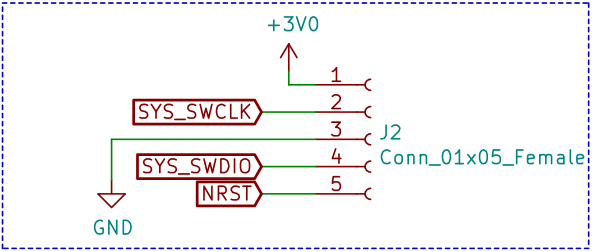
\includegraphics[scale=0.6]{img/Schematic_SWD}
	\caption{Schematic: SWD Connector}
	\label{fig:33}
\end{figure}

\section{Firmware}
The firmware that will be flashed onto the microcontroller that will be controlling the behavior of the device will be discussed in this section. The firmware is developed in the embedded C programming language. Rather than to show the developed code in this section, the finite state machine of the software will be shown to indicate the different states, and how to transition from one state to the other. This section will also show flow diagrams of the firmware that is created for the device. The state diagrams will show the different states of the device, where the flow diagrams will show the steps taken by the software during execution and the logical flow of the software.

\subsection{Finite State Machine}
A high-level state machine of the device is shown in \autoref{FSM}. In this figure, it can be seen that upon startup of the device, it will display the measured temperature of the user. The user can then press the button for less than one second to see the current time of day and press the button again for less than one second, to see the date. If the user then presses the button once again for less than one second, the temperature will be displayed again. This cycle just mentioned is the Normal Mode in which the device is operating. The current display mode will keep displaying (Self-Transition) until one transition condition is met. If this self-transition cycled for more than 5 seconds, the device will go into Standby Mode.
\\
\\
If the user wants to change the current time or date, he/she must navigate to either the time- or the date display mode and then press the button between 1.5 and 3 seconds to enter Settings Mode. In settings mode the user will cycle through all possible settings, starting at setting the hour and ending by setting the year. A short press of the button (<=1 sec) will increment the current setting, and a long press (1.5 < sec <= 3) will transition to the next setting.
\begin{figure}[H]
	\centering
	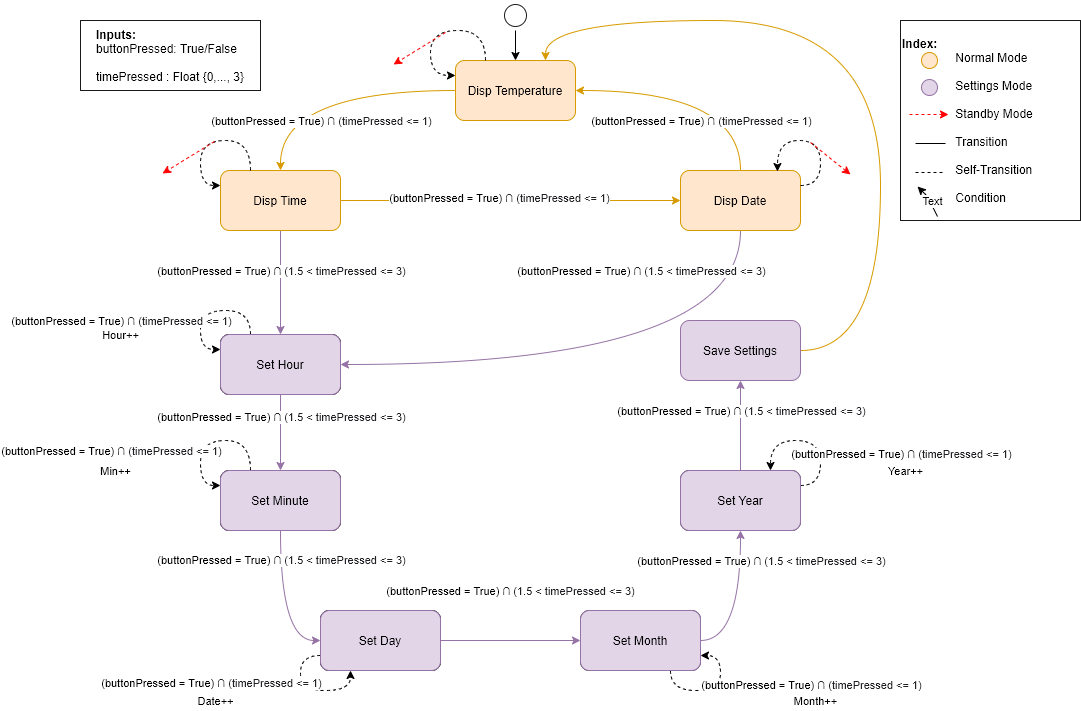
\includegraphics[scale=0.4]{img/FSM.png}
	\caption{Finite State Machine}
	\label{FSM}
\end{figure}

\subsection{Flow Diagrams}
From the FSM of the device, it is clear that there are 8 possible states that the device can be in. These states are now numbered to be referred to in the flow diagrams, and the numbering is as follow:
\begin{table}[H]
	\centering
	\caption{\textit{States of the device}}
	\label{tab:7}
	\begin{tabular}{|c|c|c|}
		\hline
		\textbf{State} & \textbf{Description} & \textbf{Mode}\\
		\hline
		\hline
		0 & Measure and Display Temperature & Normal\\
		\hline
		1 & Display Time & Normal\\
		\hline
		2 & Display Date & Normal\\
		\hline
		3 & Set Hour & Settings\\
		\hline
		4 & Set Minute & Settings\\
		\hline
		5 & Set Day & Settings\\
		\hline
		6 & Set Month & Settings\\
		\hline
		7 & Set Year & Settings\\
		\hline
	\end{tabular}
\end{table}
\noindent
The main flow diagram of the firmware is shown in \autoref{Flow-Diag1}
\begin{figure}[H]
	\centering
	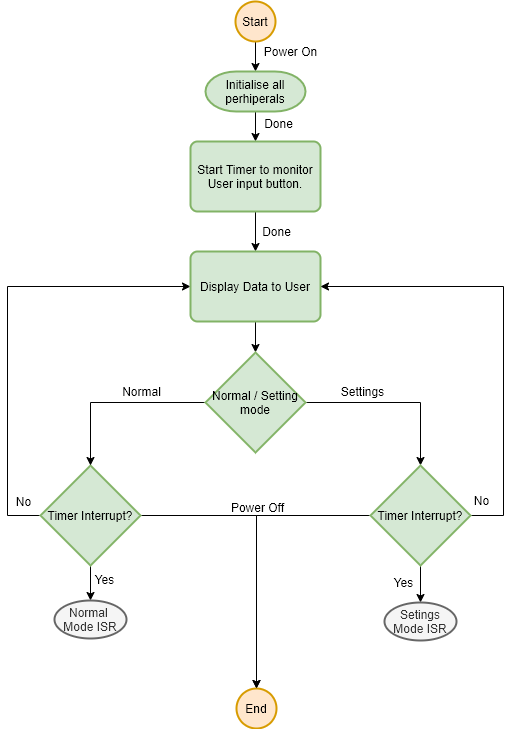
\includegraphics[scale=0.5]{img/Flow-Diag1.png}
	\caption{Main Flow Diagram}
	\label{Flow-Diag1}
\end{figure}
\noindent
From the main flow diagram of the firmware, it can be seen that when the device power-up, all the configured peripherals will be initialised. These peripherals include both I2C channels, GPIO pins, the RTC as well as all the timers used. After the peripherals are initialised, the timer used to monitor the user input button (polling) is started. Then, the requested data will be displayed to the user. On startup, the displayed data will be the user's temperature since this is the default state as seen in \autoref{FSM}. The default mode is therefore the Normal Mode. The firmware will then continuously monitor if the input button is pressed by the user. The status of the button will be monitored inside the respective mode's Interrupt Service Routine (ISR). This is demonstrated in \autoref{Flow-Diag2} and \autoref{Flow-Diag3}.
\\
\\
\autoref{Flow-Diag2} shows the flow diagram for the ISR for when in Normal Mode.
\begin{figure}[H]
	\centering
	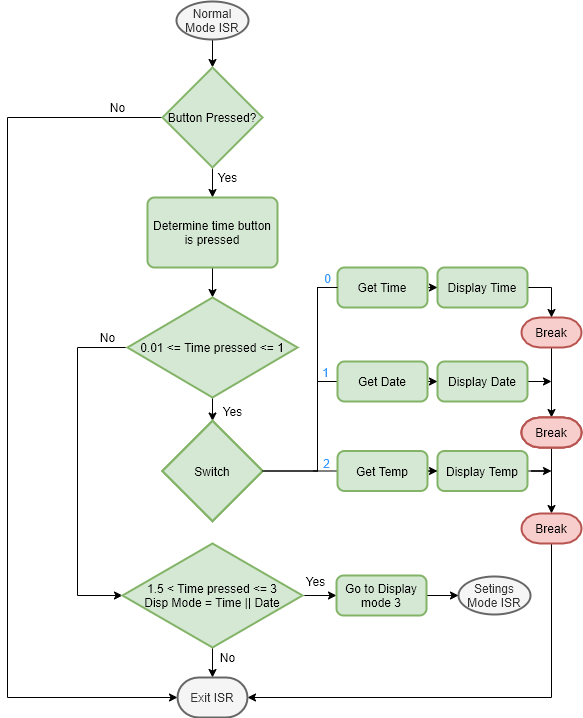
\includegraphics[scale=0.5]{img/Flow-Diag2.png}
	\caption{Normal Mode ISR}
	\label{Flow-Diag2}
\end{figure}
\noindent
From the flow diagram of the Normal Mode ISR, it can be seen that when an interrupt is triggered from \autoref{Flow-Diag1}, the firmware will determine if the button is pressed. If the button is not pressed, the firmware will return to the "Display Data to User" block of the main flow diagram. If, however, the user presses the button, the firmware will count how long the button is pressed. As mentioned earlier, if the button is pressed less than one second ( <= 1 sec), what is being displayed to the user will cycle through displaying temperature, displaying the time, and displaying the date. The blue number in the switch case refers to the current state of the device, and the corresponding green block shows to which state or display mode the device will transition into. 
\\
\\
If the button is pressed longer ( 1.5 < sec <= 3) and the current state is either to display time or date, the device will transition to Settings Mode. Settings Mode has its own ISR, and the flow diagram can be seen in \autoref{Flow-Diag3}.
\begin{figure}[H]
	\centering
	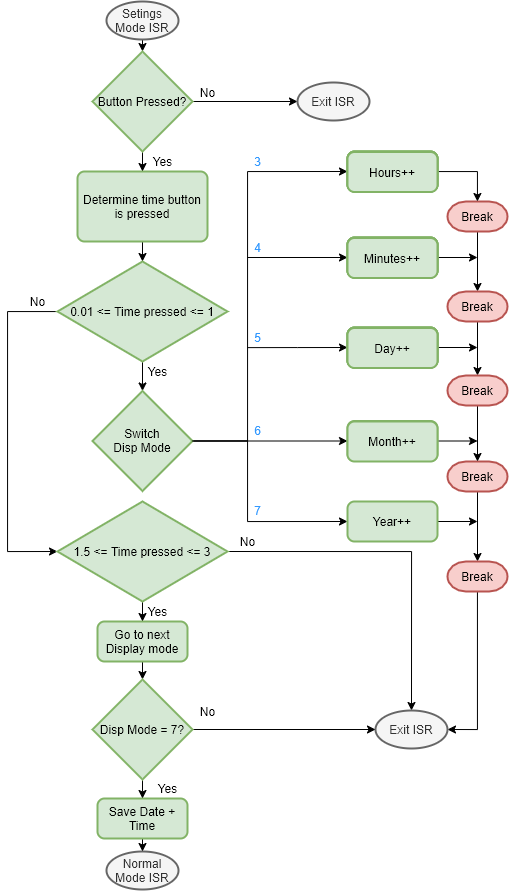
\includegraphics[scale=0.5]{img/Flow-Diag3.png}
	\caption{Settings Mode ISR}
	\label{Flow-Diag3}
\end{figure}
\noindent
Just as with the ISR for the Normal Mode, the firmware will determine if the button is pressed, and for how long the button is pressed. Once again, if the button is not pressed by the user, the firmware will return to the main flow diagram. If the button is pressed for less than one second ( <= 1 sec), the current setting that is being changed will be incremented. Therefore, if the current state is 3, the hours will be incremented, and if the current state is 4, the hours will be incremented, etc. The blue number in the switch case refers to the current state of the device. If the button is then pressed for a longer time ( 1.5 < sec <= 3), the current state will be incremented to allow the user to set the hours, minutes, date, month and year. If then the last state is reached, the newly set date and time will be saved by the firmware, and the firmware will return to Normal Mode.

\section{Concluding Remarks}
This chapter focused on the detailed design of the Body Temperature Monitoring Wristband. Components were selected by utilising Multi-Criteria Decision Matrices (MCDM) using the Weighted Product Method (WPM). Only the microcontroller, the temperature probe, battery, and display were selected in this way. The selected components can be summarised as in \autoref{tab:6}:
\begin{table}[H]
	\centering
	\caption{\textit{Component Summary}}
	\label{tab:6}
	\begin{tabular}{|c|c|}
		\hline
		\textbf{Category} & \textbf{Component} \\
		\hline
		\hline
		Microcontroller & STM32L071KBT6 \\
		\hline
		Temperature Probe & MAX30205\\
		\hline
		Display & Midas White Passive Matrix OLED Display \\
		\hline
		Battery & CR2032 Button Battery \\
		\hline
	\end{tabular}
\end{table}
\noindent
Statistical estimation was determined as the technique that will be used to estimate core body temperature from the temperature of the skin. After the component and measurement technique selections, the full schematic diagram of the designed device was given with a few design choices explained. Lastly, the firmware that will be flashed on the device was designed by means of a state machine that show the different possible states of the device and how to transition from one state to another. Firmware flow diagrams were also given to show the exact flow of the firmware, as well as the steps taken during software execution. 